% =============================================================================
%  Call Analysis — Contact Center Intelligence
%  Project Proposal (NVIDIA-green light theme)
%  Compiled with pdflatex (MiKTeX)
% =============================================================================
\documentclass[11pt,a4paper]{article}

% --- Encoding & fonts -------------------------------------------------------
\usepackage[utf8]{inputenc}
\usepackage[T1]{fontenc}
\usepackage{lmodern}

% --- Geometry ---------------------------------------------------------------
\usepackage[a4paper,margin=2.4cm,bottom=2.8cm]{geometry}

% --- Color (table option enables \rowcolor) ---------------------------------
\usepackage[table]{xcolor}

% --- NVIDIA palette ---------------------------------------------------------
\definecolor{nvidiagreen}{HTML}{76B900}      % NVIDIA signature green
\definecolor{nvidiagreendark}{HTML}{5A8F00}  % darker green (headings)
\definecolor{nvidiagreenlight}{HTML}{F3FAE2} % light green tint (boxes)
\definecolor{nvidialine}{HTML}{C9E5A0}       % soft green line
\definecolor{textdark}{HTML}{1F2933}
\definecolor{muted}{HTML}{6B7280}
\definecolor{tablehead}{HTML}{76B900}

% --- Graphics ---------------------------------------------------------------
\usepackage{tikz}
\usetikzlibrary{positioning,arrows.meta,shapes.geometric,fit,backgrounds,calc}

% --- Tables & lists ---------------------------------------------------------
\usepackage{booktabs}
\usepackage{enumitem}
\setlist{leftmargin=1.4em, itemsep=2pt, topsep=3pt}

% --- Section formatting -----------------------------------------------------
\usepackage{titlesec}
\titleformat{\section}{\Large\bfseries\color{nvidiagreendark}}{\thesection.}{0.6em}{}
\titleformat{\subsection}{\large\bfseries\color{textdark}}{\thesubsection}{0.6em}{}
\titleformat{\subsubsection}{\normalsize\bfseries\color{textdark}}{\thesubsubsection}{0.6em}{}
\titlespacing*{\section}{0pt}{14pt plus 2pt minus 2pt}{6pt}
\titlespacing*{\subsection}{0pt}{10pt plus 2pt minus 2pt}{4pt}

% --- Headers & footers ------------------------------------------------------
\usepackage{fancyhdr}
\pagestyle{fancy}
\fancyhf{}
\fancyhead[L]{\footnotesize\textcolor{nvidiagreendark}{\textbf{Call Analysis -- Contact Center Intelligence}}}
\fancyhead[R]{\footnotesize\textcolor{muted}{Project Proposal}}
\fancyfoot[C]{\small\thepage}
\renewcommand{\headrulewidth}{0.9pt}
\renewcommand{\headrule}{\color{nvidiagreen}\hrule width\headwidth height\headrulewidth}

% --- Hyperlinks -------------------------------------------------------------
\usepackage[hidelinks]{hyperref}
\hypersetup{colorlinks=true, linkcolor=nvidiagreendark, urlcolor=nvidiagreen, citecolor=nvidiagreendark}

% --- Callout boxes ----------------------------------------------------------
\usepackage[breakable,skins]{tcolorbox}
\newtcolorbox{highlight}[1][]{breakable, colback=nvidiagreenlight, colframe=nvidiagreen,
  boxrule=0.8pt, arc=2.5pt, left=2.5mm, right=2.5mm, top=1.8mm, bottom=1.8mm, #1}
\newtcolorbox{note}[1][]{breakable, colback=white, colframe=nvidialine,
  boxrule=0.8pt, arc=2.5pt, left=2.5mm, right=2.5mm, top=1.8mm, bottom=1.8mm, #1}

% --- Captions ---------------------------------------------------------------
\usepackage{caption}
\captionsetup{font=small, labelfont={bf,color=nvidiagreendark}}

% --- Misc -------------------------------------------------------------------
\usepackage{parskip}
\setlength{\parskip}{4pt}
\emergencystretch=2em

% =============================================================================
\begin{document}
\sloppy

% =============================================================================
%  TITLE PAGE
% =============================================================================
\begin{titlepage}
  \centering
  \vspace*{6mm}
  \begin{tikzpicture}[remember picture, overlay]
    \fill[nvidiagreen] (current page.north west) rectangle ([yshift=-22mm]current page.north east);
    \node[white, font=\large\bfseries] at ([yshift=-11mm]current page.north) {NVIDIA-POWERED AI PLATFORM};
  \end{tikzpicture}

  \vspace*{26mm}
  {\color{nvidiagreendark}\rule{\linewidth}{1.6pt}}\\[6mm]
  {\Huge\bfseries\color{textdark} Call Analysis}\\[4mm]
  {\LARGE\bfseries\color{nvidiagreendark} Contact Center Intelligence}\\[3mm]
  {\large\color{muted} End-to-end AI platform: Ingest $\rightarrow$ ASR $\rightarrow$ Diarization $\rightarrow$ PII Scrub $\rightarrow$ Multi-Agent Analysis $\rightarrow$ Dashboard}\\[6mm]
  {\color{nvidiagreendark}\rule{\linewidth}{1.6pt}}

  \vspace{10mm}
  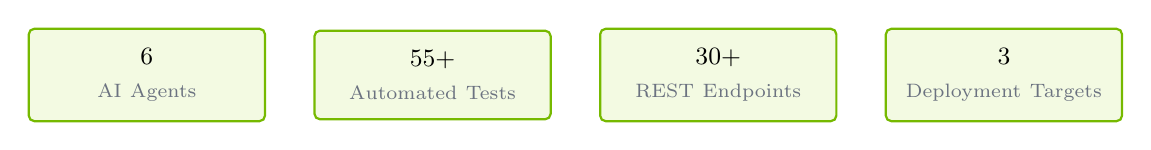
\begin{tikzpicture}[
      stat/.style={rectangle, rounded corners=2pt, draw=nvidiagreen, thick,
                   fill=nvidiagreenlight, text width=25mm, align=center,
                   inner sep=2.5mm, font=\small},
    ]
    \node[stat] (a) {6\\[1pt]{\scriptsize\textcolor{muted}{AI Agents}}};
    \node[stat, right=6mm of a] (b) {55+\\[1pt]{\scriptsize\textcolor{muted}{Automated Tests}}};
    \node[stat, right=6mm of b] (c) {30+\\[1pt]{\scriptsize\textcolor{muted}{REST Endpoints}}};
    \node[stat, right=6mm of c] (d) {3\\[1pt]{\scriptsize\textcolor{muted}{Deployment Targets}}};
  \end{tikzpicture}

  \vspace{12mm}
  {\large\bfseries\color{textdark} Project Proposal}\\[2mm]
  {\normalsize\color{muted} Version 0.4.0 \quad$\cdot$\quad Python 3.11 \quad$\cdot\quad$ FastAPI \quad$\cdot\quad$ NVIDIA NIM}

  \vfill
  {\small\color{muted} Built on the NVIDIA free AI stack (hosted NIM via \url{https://build.nvidia.com})}\\[1mm]
  {\small\color{muted} \today}
\end{titlepage}

% =============================================================================
%  TABLE OF CONTENTS
% =============================================================================
\tableofcontents
\newpage

% =============================================================================
%  1. EXECUTIVE SUMMARY
% =============================================================================
\section{Executive Summary}

\emph{Call Analysis} is an end-to-end contact center intelligence platform that turns raw
call recordings into structured, actionable insight. It combines automatic speech
recognition (ASR), multi-speaker diarization, privacy-first PII redaction, and a
orchestrated team of specialized large-language-model (LLM) agents -- all powered by
the \textbf{NVIDIA free AI stack} (hosted NIM, Llama-3.1-8B-Instruct) -- and presents
the results in an NVIDIA-themed interactive dashboard.

The platform is designed for contact center operators, QA teams, compliance officers,
and supervisors who need to answer questions such as:

\begin{itemize}
  \item How well did the agent handle this call, and what coaching would help?
  \item Did the conversation comply with policy and privacy requirements?
  \item What was the customer's sentiment and the root cause of the contact?
  \item What follow-up actions should be pushed to the CRM?
\end{itemize}

\begin{highlight}
\textbf{Key Highlights}
\begin{itemize}
  \item \textbf{6 specialized AI agents} -- QA scorecard, compliance \& risk, sentiment \&
        emotion, root cause \& intent, CRM action items, and a RAG-based call copilot.
  \item \textbf{Multi-source ingestion} -- upload recordings, or bulk-import from local
        folders, HuggingFace dataset repos, and Kaggle datasets.
  \item \textbf{Privacy by design} -- PII detection \& redaction (phones, emails, cards,
        SSN, Aadhaar, account numbers) before any LLM processing.
  \item \textbf{Production-grade core} -- FastAPI, PostgreSQL, Redis/Celery, JWT + API keys
        with RBAC, OpenTelemetry, Prometheus, Grafana, Docker Compose.
  \item \textbf{Three delivery targets} -- Docker stack, Electron Windows desktop app, and
        a standalone PyInstaller/NSIS installer.
\end{itemize}
\end{highlight}

% =============================================================================
%  2. PROBLEM STATEMENT
% =============================================================================
\section{Problem Statement}

Contact centers generate enormous volumes of recorded conversation data, yet most of it
is never analyzed. Organizations face several recurring challenges:

\begin{enumerate}
  \item \textbf{No systematic quality assurance.} Agent performance is judged by sparse,
        manual call sampling rather than continuous, consistent scoring.
  \item \textbf{Compliance exposure.} Policy violations, privacy leaks, and risky language
        are discovered after the fact -- or not at all.
  \item \textbf{Siloed insight.} Transcripts, sentiment, and action items live in separate
        tools and never feed back into coaching or CRM workflows.
  \item \textbf{High cost of AI adoption.} Many speech-to-insight solutions require
        expensive GPU infrastructure and proprietary cloud pricing.
  \item \textbf{Privacy risk.} Sending raw recordings containing personal data to LLM
        services without scrubbing is a compliance hazard (GDPR, HIPAA, local regulations).
\end{enumerate}

The goal of this project is to deliver a \textbf{complete, self-contained, low-cost}
platform that solves these problems on the NVIDIA free AI stack, deployable from a single
laptop up to a containerized production stack.

% =============================================================================
%  3. SOLUTION OVERVIEW
% =============================================================================
\section{Solution Overview}

\begin{note}
\textbf{One-line pipeline:} \emph{Ingest $\rightarrow$ ASR (Whisper) $\rightarrow$
multi-speaker diarization $\rightarrow$ PII scrub $\rightarrow$ multi-agent analysis
$\rightarrow$ NVIDIA-themed dashboard.}
\end{note}

The platform follows a modular, layered design. Each stage is an independent component
with a well-defined interface, which keeps the system testable and lets individual stages
be swapped (for example, replacing the heuristic diarizer with pyannote.audio, or switching
ASR model sizes without touching the rest of the pipeline).

\begin{highlight}
\textbf{Design principles}
\begin{itemize}
  \item \textbf{Free AI stack first} -- hosted NVIDIA NIM for LLMs; faster-whisper for ASR
        with GPU $\rightarrow$ CPU fallback.
  \item \textbf{Privacy before intelligence} -- PII is redacted before any LLM call.
  \item \textbf{Local-first, cloud-ready} -- one command on a laptop; Docker Compose for
        production; native Windows desktop distribution.
  \item \textbf{Observable by default} -- structured logging, OpenTelemetry tracing,
        Prometheus metrics, and a bundled Grafana dashboard.
\end{itemize}
\end{highlight}

% =============================================================================
%  4. SYSTEM ARCHITECTURE
% =============================================================================
\section{System Architecture}

Figure~\ref{fig:arch} shows the layered architecture. The \textbf{web dashboard} and
\textbf{Electron desktop shell} are the two presentation front-ends. Both talk to a single
\textbf{FastAPI} service that owns the domain logic: ingestion, the analysis pipeline,
agent orchestration, and the file store. Background processing is decoupled through
Celery + Redis, durable state lives in PostgreSQL, and every layer emits telemetry.

\begin{figure}[htbp]
  \centering
  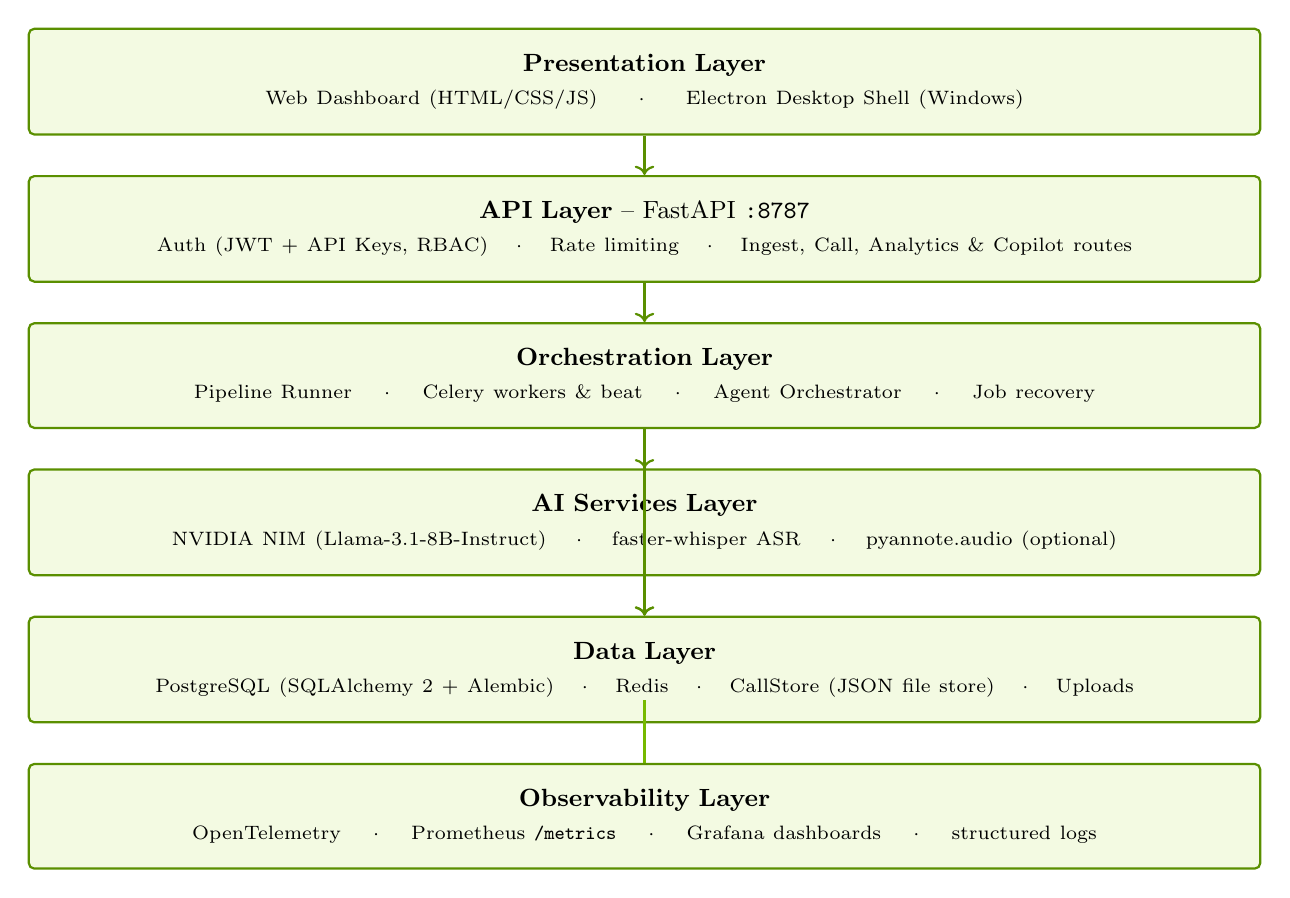
\begin{tikzpicture}[
      node distance=5mm,
      layer/.style={rectangle, draw=nvidiagreendark, thick, rounded corners=2pt,
                    fill=nvidiagreenlight, text width=150mm, align=center,
                    inner sep=3.2mm, font=\small},
      lbl/.style={font=\scriptsize\bfseries\color{muted}},
    ]
    \node[layer] (ui) {\textbf{Presentation Layer}\\[1pt]
      \scriptsize Web Dashboard (HTML/CSS/JS) $\;\cdot\;$ Electron Desktop Shell (Windows)};
    \node[layer, below=of ui] (api) {\textbf{API Layer} -- FastAPI \texttt{:8787}\\[1pt]
      \scriptsize Auth (JWT + API Keys, RBAC) $\;\cdot\;$ Rate limiting $\;\cdot\;$ Ingest, Call, Analytics \& Copilot routes};
    \node[layer, below=of api] (orch) {\textbf{Orchestration Layer}\\[1pt]
      \scriptsize Pipeline Runner $\;\cdot\;$ Celery workers \& beat $\;\cdot\;$ Agent Orchestrator $\;\cdot\;$ Job recovery};
    \node[layer, below=of orch] (ai) {\textbf{AI Services Layer}\\[1pt]
      \scriptsize NVIDIA NIM (Llama-3.1-8B-Instruct) $\;\cdot\;$ faster-whisper ASR $\;\cdot\;$ pyannote.audio (optional)};
    \node[layer, below=of ai] (data) {\textbf{Data Layer}\\[1pt]
      \scriptsize PostgreSQL (SQLAlchemy 2 + Alembic) $\;\cdot\;$ Redis $\;\cdot\;$ CallStore (JSON file store) $\;\cdot\;$ Uploads};
    \node[layer, below=of data] (obs) {\textbf{Observability Layer}\\[1pt]
      \scriptsize OpenTelemetry $\;\cdot\;$ Prometheus \texttt{/metrics} $\;\cdot\;$ Grafana dashboards $\;\cdot\;$ structured logs};

    \draw[->, thick, nvidiagreendark] (ui) -- (api);
    \draw[->, thick, nvidiagreendark] (api) -- (orch);
    \draw[->, thick, nvidiagreendark] (orch) -- (ai);
    \draw[->, thick, nvidiagreendark] (orch) -- (data);
    \draw[->, thick, nvidiagreendark] (ai) -- (data);
    \draw[-, thick, nvidiagreen] (obs.north) -- ($(data.south)+(0,3mm)$);
  \end{tikzpicture}
  \caption{Layered system architecture of the Call Analysis platform.}
  \label{fig:arch}
\end{figure}

\subsection{Component Responsibilities}

\begin{table}[htbp]
  \centering
  \small
  \begin{tabular}{@{}p{38mm}p{105mm}@{}}
    \toprule
    \rowcolor{tablehead}
    \textcolor{white}{\textbf{Component}} & \textcolor{white}{\textbf{Responsibility}} \\
    \midrule
    FastAPI service & REST API, validation (Pydantic v2), uploads, static dashboard, CORS, health checks \\
    Pipeline runner & End-to-end job orchestration: audio $\rightarrow$ report with progress \& recovery \\
    Celery + Redis & Async job queue, retries, beat scheduling, circuit breakers, job status tracking \\
    Agent orchestrator & Fans a call transcript out to 6 agents; aggregates JSON scorecards \\
    CallStore & Lightweight JSON persistence of calls, analyses, and metadata (no DB required for demo) \\
    PostgreSQL / Alembic & Multi-tenant relational persistence, users, orgs, API keys, migrations \\
    Telemetry stack & OTel traces, Prometheus metrics, Grafana dashboards, JSON logging \\
    \bottomrule
  \end{tabular}
  \caption{Primary components and their responsibilities.}
\end{table}

% =============================================================================
%  5. CORE PROCESSING PIPELINE
% =============================================================================
\section{Core Processing Pipeline}

Each uploaded recording flows through the pipeline shown in Figure~\ref{fig:pipeline}.
Stages are chained, and every stage records progress so long jobs can be resumed after a
restart (\texttt{recover\_\allowbreak interrupted\_\allowbreak jobs}).

\begin{figure}[htbp]
  \centering
  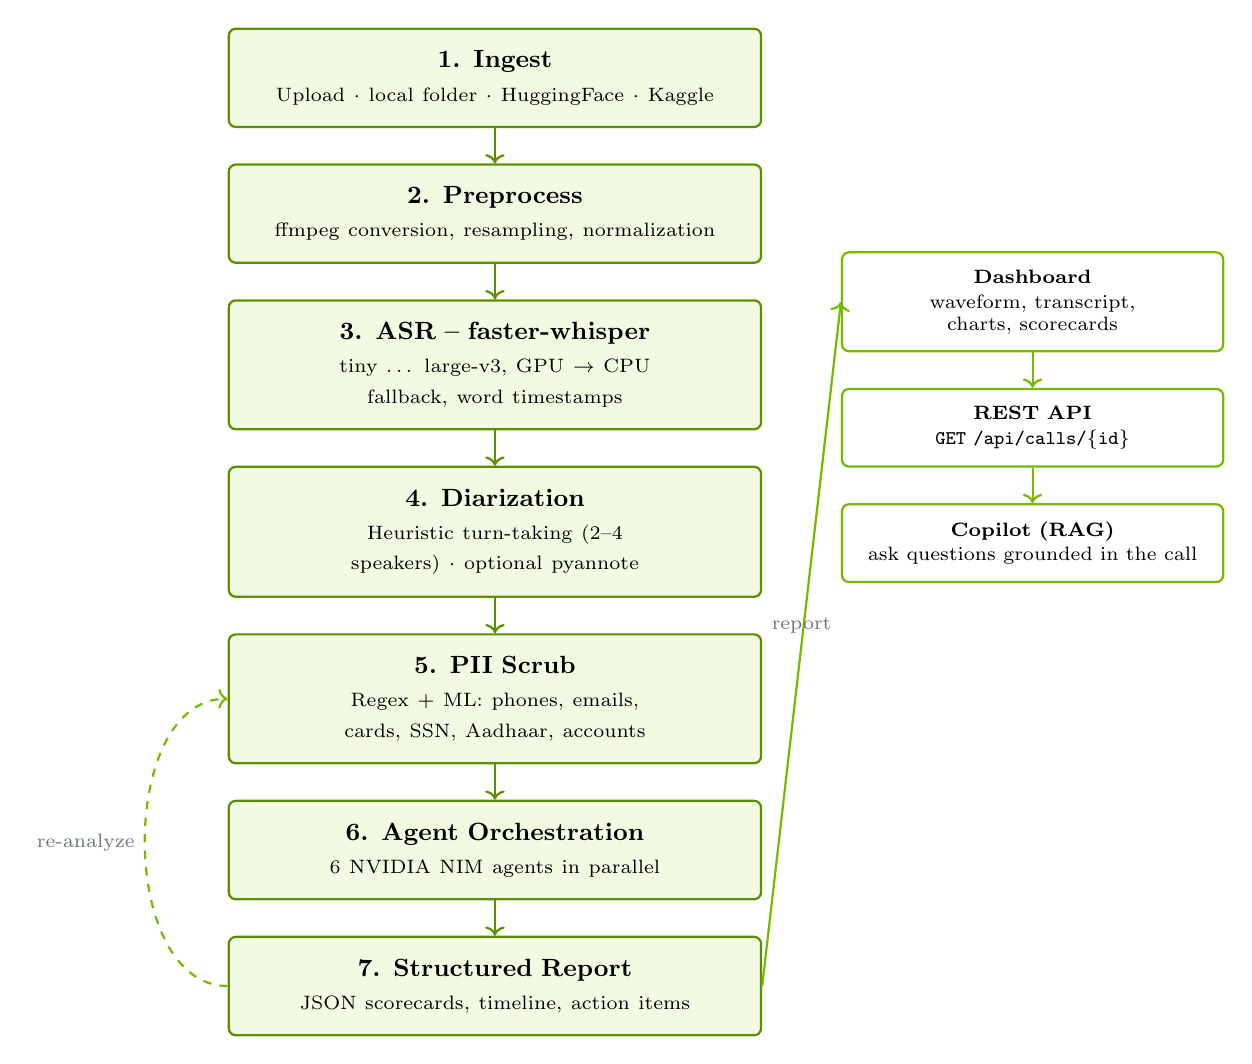
\begin{tikzpicture}[
      node distance=4.5mm,
      stage/.style={rectangle, draw=nvidiagreendark, thick, rounded corners=2.5pt,
                    fill=nvidiagreenlight, text width=62mm, align=center,
                    inner sep=2.8mm, font=\small},
      side/.style={rectangle, draw=nvidiagreen, thick, rounded corners=2.5pt,
                   fill=white, text width=44mm, align=center, inner sep=2.2mm, font=\scriptsize},
    ]
    \node[stage] (s1) {\textbf{1. Ingest}\\[1pt]\scriptsize Upload $\cdot$ local folder $\cdot$ HuggingFace $\cdot$ Kaggle};
    \node[stage, below=of s1] (s2) {\textbf{2. Preprocess}\\[1pt]\scriptsize ffmpeg conversion, resampling, normalization};
    \node[stage, below=of s2] (s3) {\textbf{3. ASR -- faster-whisper}\\[1pt]\scriptsize tiny \dots\ large-v3, GPU $\rightarrow$ CPU fallback, word timestamps};
    \node[stage, below=of s3] (s4) {\textbf{4. Diarization}\\[1pt]\scriptsize Heuristic turn-taking (2--4 speakers) $\cdot$ optional pyannote};
    \node[stage, below=of s4] (s5) {\textbf{5. PII Scrub}\\[1pt]\scriptsize Regex + ML: phones, emails, cards, SSN, Aadhaar, accounts};
    \node[stage, below=of s5] (s6) {\textbf{6. Agent Orchestration}\\[1pt]\scriptsize 6 NVIDIA NIM agents in parallel};
    \node[stage, below=of s6] (s7) {\textbf{7. Structured Report}\\[1pt]\scriptsize JSON scorecards, timeline, action items};

    \draw[->, thick, nvidiagreendark] (s1) -- (s2);
    \draw[->, thick, nvidiagreendark] (s2) -- (s3);
    \draw[->, thick, nvidiagreendark] (s3) -- (s4);
    \draw[->, thick, nvidiagreendark] (s4) -- (s5);
    \draw[->, thick, nvidiagreendark] (s5) -- (s6);
    \draw[->, thick, nvidiagreendark] (s6) -- (s7);

    \node[side, right=10mm of s3, yshift=8mm] (r1) {\textbf{Dashboard}\\[1pt]\scriptsize waveform, transcript, charts, scorecards};
    \node[side, below=of r1] (r2) {\textbf{REST API}\\[1pt]\scriptsize \texttt{GET /api/calls/\{id\}}};
    \node[side, below=of r2] (r3) {\textbf{Copilot (RAG)}\\[1pt]\scriptsize ask questions grounded in the call};

    \draw[->, thick, nvidiagreen] (s7.east) -- node[above, font=\scriptsize, color=muted]{report} ($(r1.west)+(0,0)$);
    \draw[->, thick, nvidiagreen] (r1) -- (r2);
    \draw[->, thick, nvidiagreen] (r2) -- (r3);

    \draw[->, thick, dashed, nvidiagreen] (s7.west) .. controls +(left:14mm) and +(left:14mm) ..
          node[left, font=\scriptsize, color=muted, pos=0.5]{re-analyze} (s5.west);
  \end{tikzpicture}
  \caption{End-to-end processing pipeline for a single call recording.}
  \label{fig:pipeline}
\end{figure}

\subsection{Stage Details}

\begin{table}[htbp]
  \centering
  \small
  \begin{tabular}{@{}p{30mm}p{115mm}@{}}
    \toprule
    \rowcolor{tablehead}
    \textcolor{white}{\textbf{Stage}} & \textcolor{white}{\textbf{Details}} \\
    \midrule
    Ingest & Multi-file upload; recursive folder scan; HuggingFace dataset repos (public tree API); Kaggle dataset archives (zip-slip-safe extraction, creds via env or \texttt{\textasciitilde/.kaggle/kaggle.json}); optional auto-analysis and dedupe \\
    Preprocess & ffmpeg-based conversion/normalization so downstream stages see consistent audio \\
    ASR & faster-whisper with configurable model size; GPU acceleration with automatic CPU fallback \\
    Diarization & Heuristic speaker turn-taking for 2--4 speakers; optional pyannote.audio integration \\
    PII scrub & Regex + ML detection; redaction of emails, phones, credit cards, SSN, Aadhaar, account numbers before LLM calls \\
    Agents & Parallel execution of 6 agents against the scrubbed transcript; structured JSON outputs \\
    Report & Aggregated scorecard, sentiment timeline, compliance flags, root cause, CRM actions, copilot index \\
    \bottomrule
  \end{tabular}
  \caption{Pipeline stages and implementation details.}
\end{table}

% =============================================================================
%  6. AI AGENT FRAMEWORK
% =============================================================================
\section{AI Agent Framework}

The heart of the analysis is an \textbf{agent orchestrator} that runs six specialized
LLM agents against the scrubbed transcript (Figure~\ref{fig:agents}). All agents call the
same hosted NVIDIA NIM endpoint (\texttt{Llama-3.1-8B-Instruct}) with dedicated system
prompts and JSON output contracts, so results are machine-readable and consistent.

\begin{figure}[htbp]
  \centering
  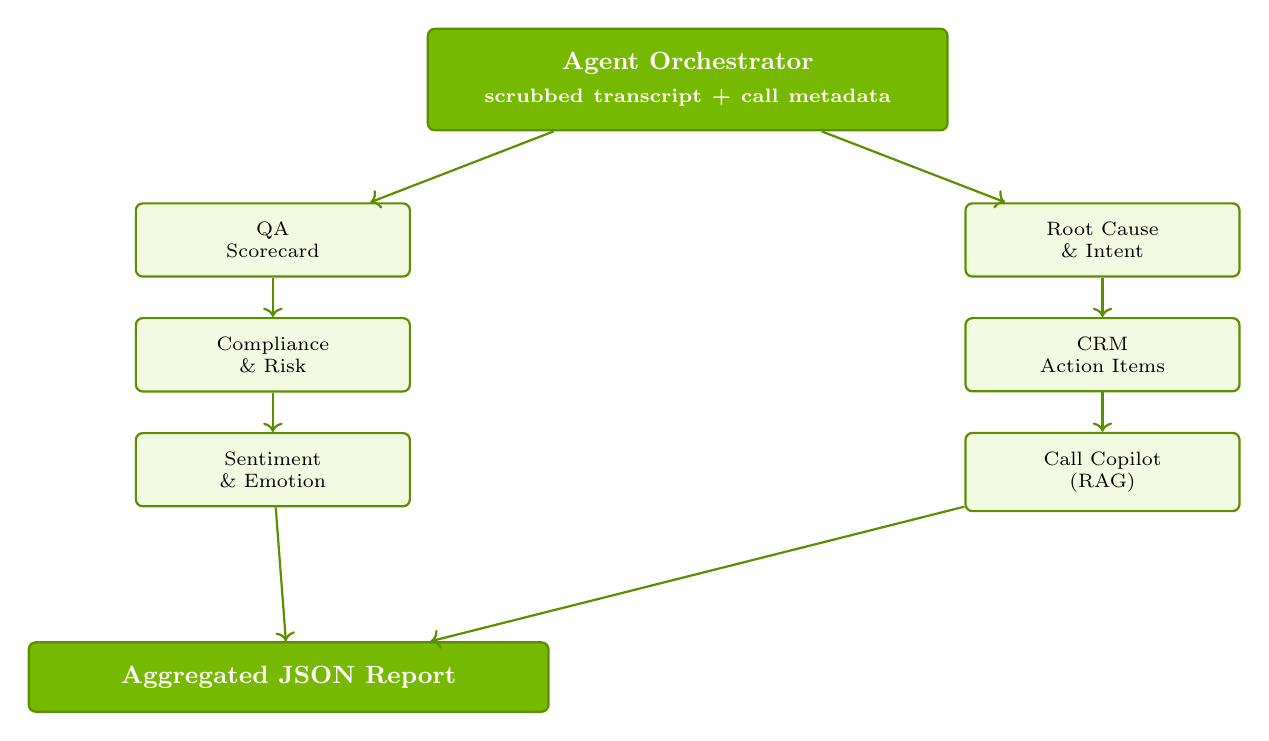
\begin{tikzpicture}[
      node distance=5mm,
      ag/.style={rectangle, draw=nvidiagreendark, thick, rounded corners=2.5pt,
                 fill=nvidiagreenlight, text width=30mm, align=center, inner sep=2.4mm, font=\scriptsize},
      hub/.style={rectangle, draw=nvidiagreendark, thick, rounded corners=2.5pt,
                  fill=nvidiagreen, text=white, text width=60mm, align=center, inner sep=3mm, font=\small\bfseries},
    ]
    \node[hub] (o) {Agent Orchestrator\\[1pt]\scriptsize\color{white} scrubbed transcript + call metadata};
    \node[ag, below left=9mm and 2mm of o] (a1) {QA\\ Scorecard};
    \node[ag, below=5mm of a1] (a2) {Compliance\\ \& Risk};
    \node[ag, below=5mm of a2] (a3) {Sentiment\\ \& Emotion};
    \node[ag, below right=9mm and 2mm of o] (a4) {Root Cause\\ \& Intent};
    \node[ag, below=5mm of a4] (a5) {CRM\\ Action Items};
    \node[ag, below=5mm of a5] (a6) {Call Copilot\\ (RAG)};
    \node[hub, below=17mm of a3, xshift=2mm] (agg) {Aggregated JSON Report};

    \draw[->, thick, nvidiagreendark] (o) -- (a1);
    \draw[->, thick, nvidiagreendark] (o) -- (a4);
    \draw[->, thick, nvidiagreendark] (a1) -- (a2);
    \draw[->, thick, nvidiagreendark] (a2) -- (a3);
    \draw[->, thick, nvidiagreendark] (a4) -- (a5);
    \draw[->, thick, nvidiagreendark] (a5) -- (a6);
    \draw[->, thick, nvidiagreendark] (a3) -- (agg);
    \draw[->, thick, nvidiagreendark] (a6) -- (agg);
  \end{tikzpicture}
  \caption{Multi-agent orchestration: one transcript, six specialized agents, one aggregated report.}
  \label{fig:agents}
\end{figure}

\begin{table}[htbp]
  \centering
  \small
  \begin{tabular}{@{}p{36mm}p{110mm}@{}}
    \toprule
    \rowcolor{tablehead}
    \textcolor{white}{\textbf{Agent}} & \textcolor{white}{\textbf{Output}} \\
    \midrule
    QA Scorecard & 0--100 performance score, structured criteria, coaching tips \\
    Compliance \& Risk & Policy/privacy violations with severity levels and evidence spans \\
    Sentiment \& Emotion & Per-turn emotional vectors and a timeline chart \\
    Root Cause \& Intent & Why the customer called; resolution status tracking \\
    CRM Action Items & Prioritized follow-ups ready to push to CRM systems \\
    Call Copilot (RAG) & Supervised Q\&A grounded in the call transcript \\
    \bottomrule
  \end{tabular}
  \caption{The six AI agents and their structured outputs.}
\end{table}

% =============================================================================
%  7. AUDIO INGESTION & DATASET SUPPORT
% =============================================================================
\section{Audio Ingestion \& Dataset Support}

Beyond single-file upload, the platform supports \textbf{bulk ingestion} from three
additional sources, making it easy to load real or synthetic call corpora for demos,
benchmarks, and pilot deployments:

\begin{table}[htbp]
  \centering
  \small
  \begin{tabular}{@{}p{34mm}p{112mm}@{}}
    \toprule
    \rowcolor{tablehead}
    \textcolor{white}{\textbf{Source}} & \textcolor{white}{\textbf{How it works}} \\
    \midrule
    Local folder & \texttt{POST /api/calls/import-folder} -- recursive scan for audio files, dedupe by filename, optional auto-analysis \\
    HuggingFace & \texttt{POST /api/calls/import-hf} -- public repo-tree API; no credentials required \\
    Kaggle & \texttt{POST /api/calls/import-kaggle} -- archive download with zip-slip-safe extraction; credentials from env or \texttt{\textasciitilde/.kaggle/kaggle.json} \\
    \bottomrule
  \end{tabular}
  \caption{Bulk ingestion sources (all also available from the dashboard \emph{Ingest} panel).}
\end{table}

Supported formats: \texttt{.m4a}, \texttt{.wav}, \texttt{.mp3}, \texttt{.ogg},
\texttt{.flac}, \texttt{.webm}, \texttt{.aac}, \texttt{.opus}. All network access uses
\texttt{httpx} (already a project dependency), so no extra packages are required.

% =============================================================================
%  8. TECHNOLOGY STACK
% =============================================================================
\section{Technology Stack}

\begin{table}[htbp]
  \centering
  \small
  \begin{tabular}{@{}p{36mm}p{110mm}@{}}
    \toprule
    \rowcolor{tablehead}
    \textcolor{white}{\textbf{Area}} & \textcolor{white}{\textbf{Technologies}} \\
    \midrule
    Web framework & Python 3.11, FastAPI, Uvicorn, Pydantic v2, pydantic-settings, httpx \\
    Database \& ORM & PostgreSQL, SQLAlchemy 2, Alembic, asyncpg, psycopg \\
    Task queue & Celery, Redis, kombu \\
    Auth \& security & python-jose (JWT), passlib/bcrypt, API keys, slowapi rate limiting \\
    Audio \& AI & faster-whisper, librosa, numpy, NVIDIA NIM (Llama-3.1-8B-Instruct), pyannote (optional) \\
    Observability & OpenTelemetry, Prometheus, Grafana, structlog, python-json-logger \\
    Packaging & Docker + Compose, PyInstaller, NSIS, Electron (desktop shell) \\
    Testing & pytest, pytest-cov, FastAPI TestClient, ruff, mypy \\
    \bottomrule
  \end{tabular}
  \caption{Technology stack by area.}
\end{table}

% =============================================================================
%  9. REST API OVERVIEW
% =============================================================================
\section{REST API Overview}

The API is grouped by domain; the full surface is self-documented at
\texttt{/docs} (Swagger UI).

\begin{table}[htbp]
  \centering
  \small
  \begin{tabular}{@{}p{52mm}p{94mm}@{}}
    \toprule
    \rowcolor{tablehead}
    \textcolor{white}{\textbf{Endpoint}} & \textcolor{white}{\textbf{Purpose}} \\
    \midrule
    \texttt{POST /api/auth/login}, \texttt{GET /api/auth/me} & JWT authentication \\
    \texttt{/api/organizations} & Multi-tenant organization CRUD (admin) \\
    \texttt{/api/users} & User management (admin) \\
    \texttt{/api/api-keys} & API key lifecycle (analyst+) \\
    \texttt{GET /api/analytics} & Fleet-level analytics \\
    \texttt{GET /api/calls}, \texttt{GET /api/calls/\{id\}} & List and inspect calls \\
    \texttt{POST /api/calls/upload} & Upload one or more recordings \\
    \texttt{POST /api/calls/import-folder | import-hf | import-kaggle} & Bulk ingestion \\
    \texttt{POST /api/calls/\{id\}/analyze} & Trigger / re-run analysis \\
    \texttt{POST /api/calls/\{id\}/copilot} & RAG copilot question \\
    \texttt{DELETE /api/calls/\{id\}} & Delete a call \\
    \texttt{/api/webhooks} & Outbound webhook management (admin) \\
    \bottomrule
  \end{tabular}
  \caption{Primary REST endpoints.}
\end{table}

% =============================================================================
%  10. SECURITY & COMPLIANCE
% =============================================================================
\section{Security \& Compliance}

\begin{itemize}
  \item \textbf{Authentication} -- JWT bearer tokens and API keys; passwords hashed with bcrypt.
  \item \textbf{Authorization (RBAC)} -- \texttt{Admin} / \texttt{Analyst} / \texttt{Viewer}
        roles; organization-scoped data isolation (multi-tenancy).
  \item \textbf{Rate limiting} -- per-client limits via slowapi to prevent abuse.
  \item \textbf{PII redaction} -- regex + ML detection scrubs personal data \emph{before}
        any LLM call; redacted transcripts are what the agents see.
  \item \textbf{Safe ingestion} -- Kaggle archives are extracted with zip-slip protection;
        dataset identifiers are validated against a strict pattern.
  \item \textbf{Hardening} -- CORS controls, security headers, input validation
        (Pydantic), structured audit events, and HTTPS guidance for production.
\end{itemize}

% =============================================================================
%  11. OBSERVABILITY & MONITORING
% =============================================================================
\section{Observability \& Monitoring}

The platform is observable by default:

\begin{itemize}
  \item \textbf{Metrics} (Prometheus, \texttt{/metrics}): \texttt{calls\_\allowbreak processed\_\allowbreak total},
        \texttt{call\_\allowbreak processing\_\allowbreak duration\_\allowbreak seconds},
        \texttt{api\_\allowbreak requests\_\allowbreak total},
        \texttt{api\_\allowbreak request\_\allowbreak duration\_\allowbreak seconds},
        \texttt{active\_jobs}, \texttt{queue\_depth}, and system metrics
        (\texttt{system\_\allowbreak cpu\_\allowbreak percent},
        \texttt{system\_\allowbreak memory\_\allowbreak percent}).
  \item \textbf{Tracing} -- OpenTelemetry instrumentation for FastAPI, SQLAlchemy, Redis,
        and httpx; OTLP exporter; bundled OpenTelemetry Collector configuration.
  \item \textbf{Dashboards} -- a Grafana dashboard ships with the repository
        (\texttt{grafana/dashboards/\allowbreak call-analysis-platform.\allowbreak json}).
  \item \textbf{Logging} -- structured JSON logs via structlog / python-json-logger.
\end{itemize}

% =============================================================================
%  12. DEPLOYMENT
% =============================================================================
\section{Deployment Options}

\subsection{Docker Compose (production stack)}

A single \texttt{docker-compose up -d} brings up PostgreSQL, Redis, the API (4 workers),
two Celery workers, Celery beat, an OpenTelemetry Collector, Prometheus, and Grafana.

\subsection{Electron Windows Desktop App}

An Electron shell spawns the Python backend as a child process, waits for
\texttt{/api/health}, and loads the dashboard in a native window. Data lives under
\texttt{\%APPDATA\%\textbackslash\allowbreak Call Analysis\textbackslash\allowbreak data}. A one-command build
pipeline (\texttt{build\_electron.py}) produces an NSIS installer
(\texttt{CallAnalysis-Setup-<version>.exe}).

\subsection{Standalone Executable}

\texttt{build\_windows.py} packages the entire backend into a single PyInstaller EXE
(\texttt{CallAnalysis.exe}) with an optional NSIS installer, for air-gapped or
non-technical deployments.

\begin{highlight}
\textbf{Developer experience} -- \texttt{python -m call\_analysis.serve} starts the full
dashboard on \texttt{http://127.0.0.1:8787} with no external services; the JSON
\texttt{CallStore} makes the demo path run on a single machine.
\end{highlight}

% =============================================================================
%  13. TESTING & QUALITY
% =============================================================================
\section{Testing \& Quality}

\begin{itemize}
  \item \textbf{Unit tests} -- 55+ tests covering API endpoints (including the ingestion
        suite), configuration, storage/models, diarization, PII redaction, and the NIM
        client (mocked).
  \item \textbf{Integration tests} -- marked \texttt{integration} for environments with
        live services (PostgreSQL, Redis, ffmpeg).
  \item \textbf{Static analysis} -- ruff (lint + import sorting) and mypy (type checking)
        enforced in CI-style workflow.
  \item \textbf{Mock-based network tests} -- HuggingFace and Kaggle flows are tested with
        \texttt{httpx.MockTransport}, so the suite is deterministic and offline.
\end{itemize}

% =============================================================================
%  14. ROADMAP & FUTURE WORK
% =============================================================================
\section{Roadmap \& Future Work}

\begin{enumerate}
  \item \textbf{Production hardening} -- wire the Celery worker to the live API path
        (Postgres-backed jobs) and complete the multi-tenant auth flow end-to-end.
  \item \textbf{More model options} -- drop-in support for additional NVIDIA NIM models
        and open-weight ASR models.
  \item \textbf{CRM integrations} -- first-class connectors (Salesforce, HubSpot) for
        action-item sync.
  \item \textbf{Real-time mode} -- streaming transcription for live-call assist.
  \item \textbf{Scale-out} -- object storage (S3/GCS) for uploads and horizontal worker
        autoscaling.
  \item \textbf{Localization} -- multilingual scorecards and compliance rules.
\end{enumerate}

% =============================================================================
%  15. CONCLUSION
% =============================================================================
\section{Conclusion}

\textbf{Call Analysis} delivers a complete, NVIDIA-powered contact center intelligence
platform: it ingests calls from files, folders, and public datasets; transcribes and
diarizes them; scrubs sensitive data; analyzes them with six specialized AI agents; and
presents everything in an interactive, NVIDIA-themed dashboard. It is testable,
observable, and ships in three deployment shapes -- Docker, a native Windows desktop app,
and a standalone executable -- all built on the NVIDIA free AI stack.

\begin{note}
\textbf{Proposal prepared by the Call Analysis team.} For a live walkthrough, run
\texttt{python -m call\_analysis.serve} and open \url{http://127.0.0.1:8787}.
\end{note}

\end{document}
